\documentclass[tikz,border=5pt]{standalone}
\usepackage{fontspec}
\setmainfont{Times New Roman}
\usepackage{unicode-math}
\setmathfont{Cambria Math}
\usetikzlibrary{shapes.geometric,positioning,fit,backgrounds,arrows.meta,calc}

\begin{document}
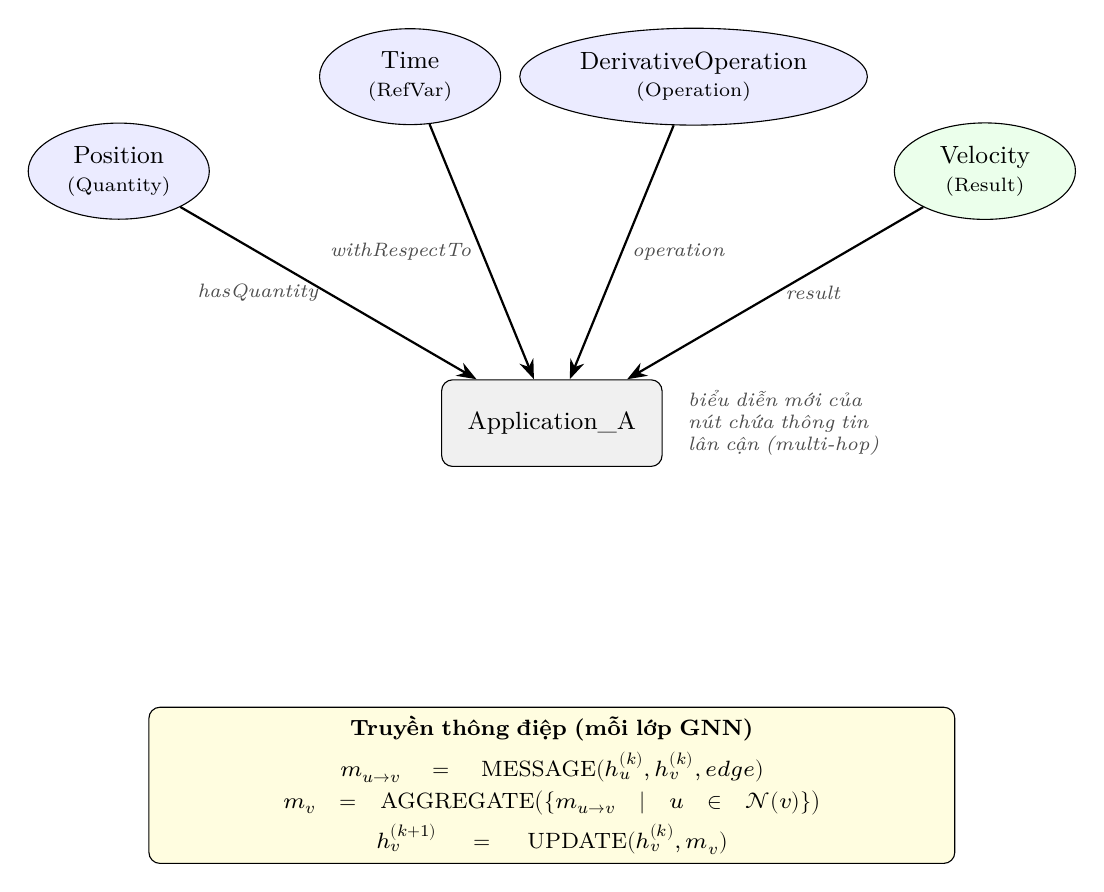
\begin{tikzpicture}[
  ent/.style={ellipse, draw, align=center, minimum width=2.3cm, minimum height=0.95cm, font=\small},
  app/.style={rectangle, draw, rounded corners, align=center, minimum height=1.1cm, font=\small},
  arrow/.style={-{Stealth[length=2.5mm]}, thick},
  label/.style={font=\scriptsize\itshape, text=gray!60!black},
]

% === Input layer (neighbors) ===
\node[ent, fill=blue!8] (pos) at (-5.5, 3.2) {Position\\[-1pt]\scriptsize (Quantity)};
\node[ent, fill=blue!8] (time) at (-1.8, 4.4) {Time\\[-1pt]\scriptsize (RefVar)};
\node[ent, fill=blue!8] (op) at (1.8, 4.4) {DerivativeOperation\\[-1pt]\scriptsize (Operation)};
\node[ent, fill=green!8] (res) at (5.5, 3.2) {Velocity\\[-1pt]\scriptsize (Result)};

% === Center node ===
\node[app, fill=gray!12, minimum width=2.8cm] (app) at (0, 0) {Application\_A};

% === Message arrows into center ===
\draw[arrow] (pos) -- node[label, left, pos=0.5] {hasQuantity} (app);
\draw[arrow] (time) -- node[label, left, pos=0.5] {withRespectTo} (app);
\draw[arrow] (op) -- node[label, right, pos=0.5] {operation} (app);
\draw[arrow] (res) -- node[label, right, pos=0.5] {result} (app);

% === Message passing inset ===
\begin{scope}[shift={(0,-4.6)}]
  \node[draw, rounded corners, fill=yellow!12, align=center, font=\footnotesize, text width=10cm]
    (mp) {%
      \textbf{Truyền thông điệp (mỗi lớp GNN)}\\[3pt]
      $m_{u \to v} = \text{MESSAGE}(h_u^{(k)}, h_v^{(k)}, edge)$\\[2pt]
      $m_v = \text{AGGREGATE}\big(\{m_{u \to v} \mid u \in \mathcal{N}(v)\}\big)$\\[2pt]
      $h_v^{(k+1)} = \text{UPDATE}(h_v^{(k)}, m_v)$
    };
\end{scope}

% === Output note ===
\node[label, right=0.2cm of app.east, align=left, text width=3.4cm]
  (out) {biểu diễn mới của\\nút chứa thông tin\\lân cận (multi-hop)};

\end{tikzpicture}
\end{document}